\chapter{Phép tính vi phân: Đạo hàm \& các quy tắc}

Ở chương trước, chúng ta đã tìm hiểu về khái niệm giới hạn và tính liên tục của hàm số. Đây là những viên gạch nền tảng để xây dựng nên một trong những công cụ mạnh mẽ và quan trọng nhất của toán học: \textbf{phép tính vi phân}.

Trọng tâm của chương này là khái niệm \textbf{đạo hàm}. Chúng ta sẽ thấy rằng đạo hàm, về bản chất, chính là cách để đo lường \textit{tốc độ thay đổi tức thời} của một đại lượng. Ý tưởng này xuất phát từ hai bài toán kinh điển: bài toán tìm hệ số góc của tiếp tuyến tại một điểm trên đường cong và bài toán xác định vận tốc tức thời của một vật chuyển động.

Trong chương này, chúng ta sẽ bắt đầu bằng việc xây dựng định nghĩa chính xác của đạo hàm từ khái niệm giới hạn. Sau đó, chúng ta sẽ phát triển một loạt các quy tắc và công thức tính toán để có thể tìm đạo hàm của nhiều loại hàm số khác nhau một cách hiệu quả, từ các hàm đơn giản đến các hàm hợp, hàm ngược và hàm ẩn. Nắm vững các kỹ thuật này sẽ là chìa khóa để chúng ta có thể ứng dụng đạo hàm vào việc khảo sát và giải quyết các bài toán thực tế trong chương tiếp theo.

\section{Đạo hàm}
\label{sec:derivative}

\subsection{Định nghĩa đạo hàm}

Trong Mục 2.1.1 của chương trước, chúng ta đã thấy rằng hai bài toán tưởng chừng không liên quan---bài toán tìm hệ số góc của tiếp tuyến và bài toán vận tốc tức thời---đều dẫn đến một khái niệm chung: giới hạn của tỉ số
$$
\dfrac{f(x) - f(a)}{x-a}
$$
khi $x$ tiến về $a$. Số thực này phản ánh tốc độ thay đổi của đại lượng $f(x)$ so với sự thay đổi của $x$.

Để củng cố ý tưởng này, chúng ta hãy xem xét lại bài toán tìm độ dốc của tiếp tuyến với đồ thị hàm số $f$ tại điểm $x_0$. Như trong Hình \ref{fig:tangent-slope}, ta có thể xấp xỉ tiếp tuyến bằng các cát tuyến $l_n$ đi qua hai điểm $(x_0, f(x_0))$ và $(x_0 + h_n, f(x_0 + h_n))$ trên đồ thị. Khi $h_n$ dần tiến về 0, các cát tuyến này sẽ tiến dần về tiếp tuyến của đồ thị tại điểm $(x_0, f(x_0))$.

Hệ số góc của cát tuyến $l_n$ được tính bởi công thức:
$$
\dfrac{f(x_0 + h_n) - f(x_0)}{(x_0 + h_n) - x_0} = \dfrac{f(x_0 + h_n) - f(x_0)}{h_n}
$$
Vì vậy, hệ số góc của tiếp tuyến chính là giới hạn của tỉ số này khi $h_n$ dần tiến về 0. Điều này dẫn chúng ta đến định nghĩa cốt lõi sau đây.

\begin{figure}[H]
	\centering
	\begin{tikzpicture}
		\begin{axis}[
			axis lines=middle,
			xmin=-1, xmax=8,
			ymin=-1, ymax=9,
			xtick={2, 3.5, 5, 6.5},
			xticklabels={$x_0$, $x_0+h_1$, $x_0+h_2$, $x_0+h_3$},
			ytick={2, 3, 4.5, 6.5},
			yticklabels={$f(x_0)$, $f(x_0+h_1)$, $f(x_0+h_2)$, $f(x_0+h_3)$},
			xlabel={},
			ylabel={},
			width=12cm,
			height=10cm,
			]
			% Define points
			\coordinate (P) at (axis cs:2,2);
			\coordinate (Q1) at (axis cs:3.5, 3);
			\coordinate (Q2) at (axis cs:5, 4.5);
			\coordinate (Q3) at (axis cs:6.5, 6.5);
			
			% % Draw secant lines
			% \addplot[domain=0:7.5, color=red, thick, samples=2, name path=l1] table {2 2 \\ 6.5 8.0625};
			% \addplot[domain=0:7.5, color=orange, thick, samples=2, name path=l2] table {2 2 \\ 5 5.5625};
			% \addplot[domain=0:7.5, color=brown, thick, samples=2, name path=l3] table {2 2 \\ 3.5 3.5625};
			
			% Draw the main function curve
			\addplot[domain=1:7, color=green!50!black, very thick, samples=100] {(1/9)*x^2 + (1/18)*x + 13/9} node[pos=0.9, right] {$f(x)$};
			
			% Draw points on the curve
			\fill (P) circle (1.5pt);
			\fill (Q1) circle (1.5pt);
			\fill (Q2) circle (1.5pt);
			\fill (Q3) circle (1.5pt);
			
			% Draw dashed lines for coordinates
			\draw[dashed] (axis cs:0, 2) -- (P);
			\draw[dashed] (axis cs:2, 0) -- (P);
			
			\draw[dashed] (axis cs:0, 3) -- (Q1);
			\draw[dashed] (axis cs:3.5, 0) -- (Q1);
			
			\draw[dashed] (axis cs:0, 4.5) -- (Q2);
			\draw[dashed] (axis cs:5, 0) -- (Q2);
			
			\draw[dashed] (axis cs:0, 6.5) -- (Q3);
			\draw[dashed] (axis cs:6.5, 0) -- (Q3);
			
			% Add labels for lines
			\node[above, color=red] at (axis cs:6, 8.5) {$l_1$};
			\node[above, color=orange] at (axis cs:5.5, 8.5) {$l_2$};
			\node[above, color=brown] at (axis cs:5, 8.5) {$l_3$};
			
		\end{axis}
	\end{tikzpicture}
	\caption{Bài toán hệ số góc của tiếp tuyến.}
	\label{fig:tangent-slope}
\end{figure}

\begin{definition}[Đạo hàm]
Cho hàm số $f$ xác định trên một khoảng mở chứa điểm $x_0$. \textbf{Đạo hàm} của $f$ tại $x_0$, ký hiệu là $f'(x_0)$, là số thực được định nghĩa bởi giới hạn:

\begin{importantbox}
    \[f'(x_0) = \limit{h}{0} \dfrac{f(x_0 + h) - f(x_0)}{h}\]
\end{importantbox}

nếu giới hạn này tồn tại. Khi đó, ta nói hàm $f$ \textbf{có đạo hàm} hay \textbf{khả vi} (differentiable) tại $x_0$.
\end{definition}

Ta cũng có thể viết lại định nghĩa đạo hàm bằng cách đặt $h = x - x_0$. Khi đó $h \to 0$ tương đương với $x \to x_0$, và ta có một dạng tương đương:

\begin{importantbox}
    \[f'(x_0) = \limit{x}{x_0} \dfrac{f(x) - f(x_0)}{x - x_0}\]
\end{importantbox}

% Nối tiếp nội dung của file chapters/03 - chapter3.tex

Một cách viết khác cũng rất phổ biến là sử dụng ký hiệu ``delta'' để biểu thị sự thay đổi. Nếu ta gọi $\Delta x = h$ là một số gia của biến $x$ tại $x_0$, thì lượng thay đổi tương ứng của giá trị hàm số $y=f(x)$ là $\Delta y = f(x_0 + \Delta x) - f(x_0)$. Khi đó, đạo hàm của $f$ tại $x_0$ chính là tỉ lệ thay đổi của $y$ so với $x$ khi $\Delta x$ vô cùng nhỏ:
$$
f'(x_0) = \limit{\Delta x}{0} \dfrac{f(x_0 + \Delta x) - f(x_0)}{\Delta x} = \limit{\Delta x}{0} \dfrac{\Delta y}{\Delta x}
$$

Vậy, đạo hàm của một hàm số tại một điểm đo lường \textbf{tốc độ thay đổi tức thời} của hàm số tại chính điểm đó. Khái niệm này là nền tảng của vô số ứng dụng trong khoa học và kỹ thuật, từ việc mô tả chuyển động của các vật thể trong vật lý đến việc tối ưu hóa lợi nhuận trong kinh tế.

Với định nghĩa chính xác về đạo hàm, giờ đây ta có thể định nghĩa một cách hình thức các khái niệm về tiếp tuyến và vận tốc đã được thảo luận trước đó.

\begin{itemize}
    \item \textbf{Tiếp tuyến:} Nếu hàm $f$ khả vi tại $x_0$, ta định nghĩa \textbf{tiếp tuyến} với đồ thị của hàm số $f$ tại điểm $P(x_0, f(x_0))$ là đường thẳng đi qua $P$ và có hệ số góc bằng $f'(x_0)$. Phương trình của tiếp tuyến này là:
    \begin{importantbox}
        \[y - f(x_0) = f'(x_0)(x - x_0)\]
    \end{importantbox}
    
    \item \textbf{Vận tốc tức thời:} Nếu $s(t)$ là hàm biểu thị vị trí của một vật trên một đường thẳng tại thời điểm $t$, và hàm $s$ khả vi tại $t_0$, thì \textbf{vận tốc tức thời} của vật tại thời điểm $t_0$ chính là $v(t_0) = s'(t_0)$.
\end{itemize}

\subsubsection{Các ví dụ tính đạo hàm bằng định nghĩa}

Bây giờ, chúng ta sẽ áp dụng định nghĩa để tính đạo hàm của một số hàm số cơ bản.

\begin{example}[Đạo hàm của hàm hằng]
Cho hàm số hằng $f(x) = c$ với mọi $x \in \R$. Hãy tìm đạo hàm của $f$.
\end{example}
\begin{solution}
Theo định nghĩa, tại một điểm $x_0$ bất kỳ:
$$
f'(x_0) = \limit{h}{0} \dfrac{f(x_0 + h) - f(x_0)}{h} = \limit{h}{0} \dfrac{c - c}{h} = \limit{h}{0} 0 = 0
$$
Vậy, $f'(x_0) = 0$ với mọi $x_0 \in \R$. Kết quả này hoàn toàn phù hợp với trực giác: một đại lượng không đổi thì có tốc độ thay đổi bằng 0.
\end{solution}

\begin{example}[Đạo hàm của hàm đồng nhất]
Tính đạo hàm của hàm số $f(x) = x$ tại một điểm $x_0$ bất kỳ.
\end{example}
\begin{solution}
Ta có:
$$
f'(x_0) = \limit{h}{0} \dfrac{f(x_0 + h) - f(x_0)}{h} = \limit{h}{0} \dfrac{(x_0 + h) - x_0}{h} = \limit{h}{0} \dfrac{h}{h} = \limit{h}{0} 1 = 1
$$
Vậy $f'(x_0) = 1$. Về mặt hình học, đồ thị của $y=x$ là một đường thẳng có hệ số góc bằng 1, nên tiếp tuyến tại mọi điểm trùng với chính nó và cũng có hệ số góc bằng 1.
\end{solution}

\begin{example}[Đạo hàm của hàm bậc hai]
Sử dụng định nghĩa, hãy tính đạo hàm của hàm số $f(x) = x^2$ tại điểm $x=x_0$.
\end{example}
\begin{solution}
Đầu tiên, ta tính số gia của hàm số:
$$
f(x_0 + h) - f(x_0) = (x_0 + h)^2 - x_0^2 = (x_0^2 + 2x_0h + h^2) - x_0^2 = 2x_0h + h^2
$$
Do đó, tỉ số của số gia là:
$$
\dfrac{f(x_0 + h) - f(x_0)}{h} = \dfrac{2x_0h + h^2}{h} = 2x_0 + h
$$
Lấy giới hạn khi $h \to 0$, ta được:
$$
f'(x_0) = \limit{h}{0} (2x_0 + h) = 2x_0
$$
Điều này có nghĩa là hàm $f(x) = x^2$ có đạo hàm tại mọi điểm $x_0$, và $f'(x_0) = 2x_0$.
\end{solution}

\begin{example}[Đạo hàm của hàm lũy thừa $f(x) = x^k$]
Với $k$ là một số nguyên dương, hãy tính đạo hàm của hàm $f(x) = x^k$ tại $x=x_0$.
\end{example}
\begin{solution}
Ta cần tính giới hạn của tỉ số $\dfrac{(x_0+h)^k - x_0^k}{h}$. Sử dụng công thức nhị thức Newton, ta có:
$$
(x_0+h)^k = x_0^k + kx_0^{k-1}h + \dfrac{k(k-1)}{2!}x_0^{k-2}h^2 + \dots + h^k
$$
Do đó:
\begin{align*}
\dfrac{(x_0+h)^k - x_0^k}{h} &= \dfrac{(x_0^k + kx_0^{k-1}h + \dots + h^k) - x_0^k}{h} \\
&= \dfrac{kx_0^{k-1}h + \dfrac{k(k-1)}{2!}x_0^{k-2}h^2 + \dots + h^k}{h} \\
&= kx_0^{k-1} + \dfrac{k(k-1)}{2!}x_0^{k-2}h + \dots + h^{k-1}
\end{align*}
Khi cho $h \to 0$, tất cả các số hạng chứa $h$ sẽ tiến về 0. Vì vậy:
$$
f'(x_0) = \limit{h}{0} \left( kx_0^{k-1} + \dfrac{k(k-1)}{2!}x_0^{k-2}h + \dots + h^{k-1} \right) = kx_0^{k-1}
$$
Vậy, $(x^k)' = kx^{k-1}$.
\end{solution}

\begin{example}[Đạo hàm của hàm căn thức]
Tính đạo hàm của hàm số $f(x) = \sqrt{x}$ (với $x > 0$).
\end{example}
\begin{solution}
Ta tính giới hạn bằng phương pháp nhân lượng liên hợp:
\begin{align*}
f'(x) = \limit{h}{0} \dfrac{\sqrt{x+h} - \sqrt{x}}{h} &= \limit{h}{0} \dfrac{(\sqrt{x+h} - \sqrt{x})(\sqrt{x+h} + \sqrt{x})}{h(\sqrt{x+h} + \sqrt{x})} \\
&= \limit{h}{0} \dfrac{(x+h) - x}{h(\sqrt{x+h} + \sqrt{x})} \\
&= \limit{h}{0} \dfrac{h}{h(\sqrt{x+h} + \sqrt{x})} \\
&= \limit{h}{0} \dfrac{1}{\sqrt{x+h} + \sqrt{x}} = \dfrac{1}{2\sqrt{x}}
\end{align*}
Giới hạn này tồn tại với mọi $x > 0$. Vậy, $(\sqrt{x})' = \dfrac{1}{2\sqrt{x}}$.
\end{solution}

\subsubsection{Đạo hàm như một hàm số}

Qua các ví dụ trên, ta thấy rằng để tìm công thức chung cho đạo hàm, việc định nghĩa đạo hàm như một hàm số mới sẽ tiện lợi hơn. Thay vì tính đạo hàm tại từng điểm $x_0$ riêng lẻ, ta định nghĩa \textbf{hàm đạo hàm} $f'$ có giá trị tại mỗi điểm $x$ là $f'(x)$.

\begin{tcolorbox}[colback=yellow!10!white, colframe=blue!75!black, fonttitle=\bfseries, boxrule=0.5pt, arc=2mm]
$$
f'(x) = \limit{h}{0} \dfrac{f(x+h) - f(x)}{h}
$$
\end{tcolorbox}

Cách tiếp cận này không chỉ giúp ta không cần giới thiệu thêm biến $x_0$ mà còn làm nổi bật vai trò của đạo hàm như một hàm số mới, được ``dẫn xuất'' từ hàm ban đầu.\footnote{Từ ``đạo hàm'' có thể có nghĩa sơ lược là đường hướng của hàm, có lẽ bắt nguồn từ thuật ngữ ban đầu mà Newton đưa ra là \textit{fluxion}. Ngày nay thuật ngữ đạo hàm trong tiếng Anh là \textit{derivative}, có nghĩa là dẫn xuất, từ một cái khác mà ra.}

Trong định nghĩa đạo hàm tại một điểm $x_0$, để thuận tiện ta yêu cầu điểm $x_0$ phải có một khoảng mở chứa nó nằm trong miền xác định của hàm. Mặc dù vậy, theo định nghĩa của giới hạn, để xét giới hạn trong định nghĩa đạo hàm thì giả thiết $x_0$ là một điểm tụ của miền xác định là đủ. Đôi khi yêu cầu ít hơn này được sử dụng, chẳng hạn nếu hàm xác định trên đoạn $[a, b]$ thì ta có thể định nghĩa \textbf{đạo hàm bên phải} tại $a$ (chỉ xét giới hạn bên phải) và \textbf{đạo hàm bên trái} tại $b$ (chỉ xét giới hạn bên trái).

\subsection{Liên hệ giữa khả vi và liên tục}

Một câu hỏi tự nhiên được đặt ra là: Mối liên hệ giữa một hàm số có đạo hàm và một hàm số liên tục là gì? Một cách trực quan, để một đồ thị có tiếp tuyến tại một điểm, nó không thể bị ``đứt'' hay có ``lỗ hổng'' tại điểm đó. Điều này gợi ý rằng tính khả vi là một điều kiện mạnh hơn tính liên tục.

Ta nói hàm số $f$ là \textbf{khả vi} (có vi phân) tại $x$ nếu $f$ có đạo hàm tại $x$. Ta có thể đoán rằng để $f$ khả vi tại $x$, tức là để tỉ số $\dfrac{f(x+h)-f(x)}{h}$ có giới hạn khi $h$ tiến về 0, thì tử số $f(x+h)-f(x)$ phải tiến về 0. Điều này có nghĩa là hàm $f$ phải liên tục tại $x$. Thật vậy, ta có định lý quan trọng sau đây.

\begin{theorem}[Khả vi thì liên tục]
Nếu hàm số $f$ khả vi tại $x$ thì $f$ liên tục tại $x$.
\end{theorem}

\begin{proof}
Giả sử $f$ có đạo hàm tại $x$. Ta cần chứng minh $f$ liên tục tại $x$, tức là $\limit{h}{0} f(x+h) = f(x)$.
Ta có thể viết lại $f(x+h) - f(x)$ như sau:
$$
f(x+h) - f(x) = \dfrac{f(x+h) - f(x)}{h} \cdot h, \quad (\text{với } h \neq 0)
$$
Lấy giới hạn hai vế khi $h \to 0$, ta được:
\begin{align*}
\limit{h}{0} [f(x+h) - f(x)] &= \limit{h}{0} \left[ \dfrac{f(x+h) - f(x)}{h} \cdot h \right] \\
&= \left( \limit{h}{0} \dfrac{f(x+h) - f(x)}{h} \right) \cdot \left( \limit{h}{0} h \right) \\
&= f'(x) \cdot 0 = 0
\end{align*}
Từ đó suy ra $\limit{h}{0} f(x+h) = f(x)$, vậy $f$ liên tục tại $x$.
\end{proof}

Mệnh đề phản đảo là ``không liên tục thì không khả vi''. Về mặt hình học, một hàm số không khả vi tại một điểm nếu đồ thị của nó bị ``đứt'' (không liên tục), hoặc nếu đồ thị ``liền mạch'' nhưng có một ``góc nhọn'' tại điểm đó.
% TODO: Chèn Hình 3.1.2: Các trường hợp đồ thị của hàm số không khả vi.

Điều quan trọng cần nhấn mạnh là mệnh đề đảo của định lý trên không đúng: \textbf{liên tục không suy ra khả vi}. Một hàm số có thể liên tục tại một điểm nhưng không có đạo hàm tại điểm đó.

\begin{example}[Hàm liên tục nhưng không khả vi]
Xét hàm giá trị tuyệt đối $f(x) = |x|$.
Ta biết rằng hàm này liên tục trên $\R$. Tuy nhiên, tại $x=0$, đồ thị của hàm có một góc nhọn (xem Hình \ref{fig:abs_value_graph}). Ta sẽ chứng tỏ hàm không có đạo hàm tại điểm này.
Xét giới hạn của tỉ số $\dfrac{f(0+h) - f(0)}{h} = \dfrac{|h|}{h}$ khi $h \to 0$.
\begin{itemize}
    \item \textbf{Giới hạn bên phải:} $\limit{h}{0^+} \dfrac{|h|}{h} = \limit{h}{0^+} \dfrac{h}{h} = 1$.
    \item \textbf{Giới hạn bên trái:} $\limit{h}{0^-} \dfrac{|h|}{h} = \limit{h}{0^-} \dfrac{-h}{h} = -1$.
\end{itemize}
Vì giới hạn bên trái và giới hạn bên phải khác nhau, nên giới hạn $\limit{h}{0} \dfrac{|h|}{h}$ không tồn tại. Do đó, hàm $f(x)=|x|$ không có đạo hàm tại $x=0$ mặc dù nó liên tục tại đó.
\end{example}

\begin{figure}[H]
    \centering
    \begin{tikzpicture}[scale=0.8]
        \begin{axis}[
            axis lines=middle,
            xmin=-3.5, xmax=3.5,
            ymin=-0.5, ymax=3.5,
            xtick=\empty,
            ytick=\empty,
            clip=false
        ]
        \addplot[domain=-3:3, thick, teal] {abs(x)};
        \node[teal] at (axis cs: 2.5, 1.5) {$f(x) = |x|$};
        \end{axis}
    \end{tikzpicture}
    \caption{\centering Đồ thị của hàm $f(x)=|x|$ có một góc nhọn tại 0 nên liên tục mà không khả vi.}
    \label{fig:abs_value_graph}
\end{figure}

\subsection{Tính chất của đạo hàm}

Việc tính đạo hàm trực tiếp từ định nghĩa có thể trở nên phức tạp. May mắn thay, có những quy tắc cho phép chúng ta tính đạo hàm của các hàm phức tạp từ các hàm đơn giản hơn.

\begin{theorem}[Các quy tắc tính đạo hàm]
Giả sử $f$ và $g$ là các hàm số có đạo hàm tại $x$, và $\alpha$ là một hằng số thực. Khi đó, các hàm $f+g$, $f-g$, $\alpha \cdot f$, $f \cdot g$ và $\dfrac{f}{g}$ (nếu $g(x) \neq 0$) cũng có đạo hàm tại $x$, và ta có các công thức sau:
\begin{enumerate}[label=(\alph*)]
    \item \[(f+g)'(x) = f'(x) + g'(x)\]
    \item \[(f-g)'(x) = f'(x) - g'(x)\]
    \item \[(\alpha \cdot f)'(x) = \alpha f'(x)\]
    \item \[(f \cdot g)'(x) = f'(x)g(x) + f(x)g'(x)\]
    \item \[\left(\dfrac{f}{g}\right)'(x) = \dfrac{f'(x)g(x) - f(x)g'(x)}{[g(x)]^2}\]
\end{enumerate}
\end{theorem}

\begin{proof}
Ta sẽ chứng minh các quy tắc (a), (d), và (e) bằng cách sử dụng định nghĩa đạo hàm. Các quy tắc còn lại có thể được chứng minh tương tự.

\textbf{(a) Quy tắc tổng:}
\begin{align*}
(f+g)'(x) &= \limit{h}{0} \dfrac{(f+g)(x+h) - (f+g)(x)}{h} \\
&= \limit{h}{0} \dfrac{[f(x+h) + g(x+h)] - [f(x) + g(x)]}{h} \\
&= \limit{h}{0} \left[ \dfrac{f(x+h) - f(x)}{h} + \dfrac{g(x+h) - g(x)}{h} \right] \\
&= \limit{h}{0} \dfrac{f(x+h) - f(x)}{h} + \limit{h}{0} \dfrac{g(x+h) - g(x)}{h} \\
&= f'(x) + g'(x)
\end{align*}

\textbf{(d) Quy tắc nhân:}
Để chứng minh quy tắc nhân, ta sử dụng một kỹ thuật là thêm bớt một số hạng ở tử số:
\begin{align*}
(f \cdot g)'(x) &= \limit{h}{0} \dfrac{f(x+h)g(x+h) - f(x)g(x)}{h} \\
&= \limit{h}{0} \dfrac{f(x+h)g(x+h) - f(x)g(x+h) + f(x)g(x+h) - f(x)g(x)}{h} \\
&= \limit{h}{0} \left[ \dfrac{f(x+h) - f(x)}{h} \cdot g(x+h) + f(x) \cdot \dfrac{g(x+h) - g(x)}{h} \right] \\
&= \left(\limit{h}{0} \dfrac{f(x+h) - f(x)}{h}\right) \cdot \left(\limit{h}{0} g(x+h)\right) + \left(\limit{h}{0} f(x)\right) \cdot \left(\limit{h}{0} \dfrac{g(x+h) - g(x)}{h}\right) \\
&= f'(x)g(x) + f(x)g'(x)
\end{align*}
Ở bước cuối, ta đã sử dụng tính liên tục của $g$ tại $x$ (vì $g$ khả vi tại $x$), tức là $\limit{h}{0} g(x+h) = g(x)$.

\textbf{(e) Quy tắc chia:}
\begin{align*}
\left(\dfrac{f}{g}\right)'(x) &= \limit{h}{0} \dfrac{\dfrac{f(x+h)}{g(x+h)} - \dfrac{f(x)}{g(x)}}{h} \\
&= \limit{h}{0} \dfrac{f(x+h)g(x) - f(x)g(x+h)}{h \cdot g(x+h)g(x)} \\
&= \limit{h}{0} \dfrac{f(x+h)g(x) - f(x)g(x) + f(x)g(x) - f(x)g(x+h)}{h \cdot g(x+h)g(x)} \\
&= \limit{h}{0} \dfrac{1}{g(x+h)g(x)} \left[ \dfrac{f(x+h)-f(x)}{h}g(x) - f(x)\dfrac{g(x+h)-g(x)}{h} \right] \\
&= \dfrac{1}{[g(x)]^2} \left[ f'(x)g(x) - f(x)g'(x) \right] = \dfrac{f'(x)g(x) - f(x)g'(x)}{[g(x)]^2}
\end{align*}
\end{proof}

\begin{example}
Sử dụng các quy tắc trên để tính đạo hàm của các hàm số sau.
\begin{enumerate}[label=(\alph*)]
    \item $f(x) = x^8 + 12x^5 - 4x^4 + 10x - 7$
    \begin{solution}
    \begin{align*}
    f'(x) &= (x^8)' + (12x^5)' - (4x^4)' + (10x)' - (7)' \\
    &= 8x^7 + 12(5x^4) - 4(4x^3) + 10(1) - 0 \\
    &= 8x^7 + 60x^4 - 16x^3 + 10
    \end{align*}
    \end{solution}
    
    \item $g(x) = (x^3 + 2x - 1)(x^2 - 5)$
    \begin{solution}
    Áp dụng quy tắc nhân:
    \begin{align*}
    g'(x) &= (x^3 + 2x - 1)'(x^2 - 5) + (x^3 + 2x - 1)(x^2 - 5)' \\
    &= (3x^2 + 2)(x^2 - 5) + (x^3 + 2x - 1)(2x) \\
    &= (3x^4 - 15x^2 + 2x^2 - 10) + (2x^4 + 4x^2 - 2x) \\
    &= 5x^4 - 9x^2 - 2x - 10
    \end{align*}
    \end{solution}
    
    \item $h(x) = \dfrac{x^2 - 3}{x^2 + 3}$
    \begin{solution}
    Áp dụng quy tắc chia:
    \begin{align*}
    h'(x) &= \dfrac{(x^2 - 3)'(x^2 + 3) - (x^2 - 3)(x^2 + 3)'}{(x^2 + 3)^2} \\
    &= \dfrac{(2x)(x^2 + 3) - (x^2 - 3)(2x)}{(x^2 + 3)^2} \\
    &= \dfrac{2x^3 + 6x - 2x^3 + 6x}{(x^2 + 3)^2} = \dfrac{12x}{(x^2 + 3)^2}
    \end{align*}
    \end{solution}
\end{enumerate}
\end{example}

\subsection{Bài tập}

\begin{exercise}
Bằng ý nghĩa hình học của đạo hàm, hãy giải thích vì sao đạo hàm của hàm số hằng bằng 0, và đạo hàm của hàm số tuyến tính $f(x) = mx + b$ bằng $m$.
\end{exercise}

\begin{exercise}
Cho hàm số $f(x) = 2x^2 - 1$. Cho hai điểm $P=(1, 1)$ và $Q=(1+h, f(1+h))$, với $h \neq 0$, thuộc đồ thị của $f$.
\begin{enumerate}[label=(\alph*)]
    \item Tính theo $h$ hệ số góc của cát tuyến $PQ$.
    \item Sử dụng định nghĩa, tính hệ số góc của tiếp tuyến tại $P$.
\end{enumerate}
\end{exercise}

\begin{exercise}
Hãy giải thích ý nghĩa của $f'(500) = 5$, nếu:
\begin{enumerate}[label=(\alph*)]
    \item $f(t)$ là vị trí của một chiếc xe (theo mét) tại thời điểm $t$ (theo giây).
    \item $f(x)$ là lợi nhuận (theo triệu đồng) khi bán được $x$ nghìn sản phẩm.
\end{enumerate}
\end{exercise}

\begin{exercise}
Dùng định nghĩa của đạo hàm, tính đạo hàm của các hàm số sau:
\begin{enumerate}[label=(\alph*)]
    \item $f(x) = x^3$
    \item $f(x) = \dfrac{1}{x+1}$
    \item $f(x) = \sqrt{2x+1}$
\end{enumerate}
\end{exercise}

\begin{exercise}
Dựa vào các đồ thị đã cho trong Hình~\ref{fig:exercise_continuity_graph} và Hình~\ref{fig:complex_piecewise_graph}, hãy tìm các điểm tại đó hàm số không khả vi và giải thích tại sao (ví dụ: điểm gián đoạn, điểm có góc nhọn, hoặc điểm có tiếp tuyến thẳng đứng). \footnote{Lưu ý rằng các khái niệm về tính liên tục và tính khả vi của một hàm số chỉ được xét tại các điểm thuộc tập xác định của hàm số đó.}
\end{exercise}

\begin{figure}[H]
    \centering
    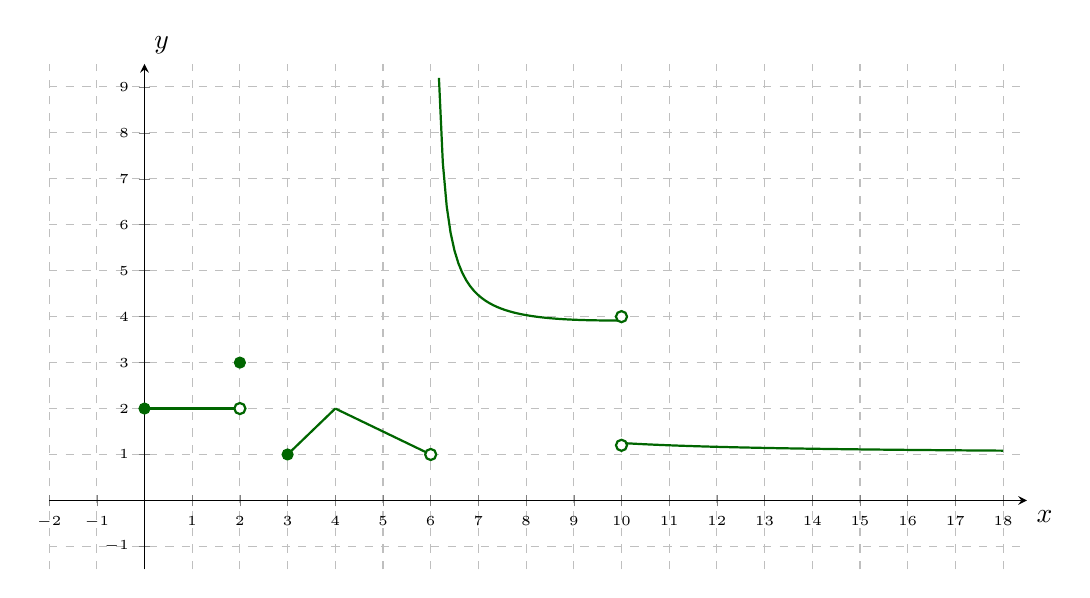
\begin{tikzpicture}
        \begin{axis}[
            axis lines=middle,
            xlabel=$x$,
            ylabel=$y$,
            xmin=-2, xmax=18.5,
            ymin=-1.5, ymax=9.5,
            grid=major,
            grid style={dashed, gray!50},
            xtick={-2,-1,0,1,...,18},
            ytick={-1,0,1,...,9},
            width=14cm,
            height=8cm,
            tick label style={font=\tiny},
            xlabel style={anchor=north west},
            ylabel style={anchor=south west},
            no markers % Tắt các marker tự động
        ]
            % Định nghĩa màu sắc cho đồ thị
            \colorlet{mygreen}{green!40!black}

            % --- Vẽ các đoạn của hàm số ---
            
            % 1. Đoạn ngang y=2, từ x=0 đến x=2
            \addplot[mygreen, thick, domain=0:2] {2};

            % 2. Hình chữ V, từ (3,1) đến (4,2) rồi đến (6,1)
            \addplot[mygreen, thick, domain=3:4] {x-2};
            \addplot[mygreen, thick, domain=4:6] {-0.5*x + 4};

            % 3. Nhánh Hyperbola với tiệm cận đứng x=6
            % Vẽ phần gần tiệm cận, giới hạn chiều cao để không bị vỡ hình
            \addplot[mygreen, thick, domain=6.01:10, samples=50, restrict y to domain=-1.5:10.5] {1/(x-6) + 1/15*x + 3};
            % Vẽ phần còn lại của nhánh hyperbola
            \addplot[mygreen, thick, domain=10:18, samples=50] {1/(x-6) + 1};

            % --- Đánh dấu các điểm đặc biệt ---
            
            % Các điểm được tô đầy (included)
            \addplot[only marks, mark=*, mygreen, mark size=2pt, fill=mygreen] coordinates {
                (0,2)   % Điểm bắt đầu của đoạn ngang
                (2,3)   % Điểm riêng lẻ ở trên
                (3,1)   % Điểm bắt đầu của hình chữ V
            };

            % Các điểm rỗng (excluded)
            \addplot[only marks, mark=o, mygreen, mark size=2pt, draw=mygreen, fill=white, thick] coordinates {
                (2,2)   % Điểm kết thúc của đoạn ngang
                (6,1)   % Điểm kết thúc của hình chữ V
                (10,4)   % Điểm bị loại trừ trên nhánh hyperbola
                (10,1.2) % Điểm bị loại trừ trên nhánh hyperbola
            };

        \end{axis}
    \end{tikzpicture}
    \caption{Hình 3.1.4}
    \label{fig:complex_piecewise_graph}
\end{figure}


\begin{exercise}
Hãy phác họa đồ thị của mỗi hàm số sau đây, và khảo sát tính liên tục hay khả vi của mỗi hàm tại điểm nối.
\begin{enumerate}[label=(\alph*)]
    \item $y = \begin{cases} x^2, & x \le 1, \\ 2x-1, & x > 1. \end{cases}$ \quad (liên tục và khả vi)
    \item $y = \begin{cases} x^2+1, & x \ge 0, \\ x+1, & x < 0. \end{cases}$ \quad (liên tục nhưng không khả vi)
\end{enumerate}
\end{exercise}

\begin{exercise}
Xét $f(x) = \sqrt[3]{x}$. Chứng tỏ rằng $f'(0)$ không tồn tại. Đây là trường hợp tiếp tuyến thẳng đứng. Hãy vẽ đồ thị để minh họa.
\end{exercise}

\begin{exercise}
Xét $f(x) = \sqrt[3]{x^2}$. Chứng tỏ rằng $f'(0)$ không tồn tại. Đây là trường hợp đồ thị có một điểm nhọn (cusp). Hãy vẽ đồ thị để minh họa.
\end{exercise}

\begin{exercise}
Chứng tỏ rằng hàm số $f(x) = |x-6|$ liên tục tại mọi nơi nhưng không khả vi tại $x=6$. Hãy phác họa đồ thị của hàm số này.
\end{exercise}

\begin{exercise}
Cho hàm số $f(x) = \begin{cases} x+1, & x \le 1 \\ 3-x, & 1 < x < 2 \\ \dfrac{1}{x-1}, & x \ge 2. \end{cases}$. Hàm số này khả vi tại những điểm nào? Giải thích.
\end{exercise}
\section{Các công thức cho đạo hàm}
\subsection{Đạo hàm của hàm hợp}

Giả sử ta muốn tính đạo hàm của hàm số $y = \sin(x^3 + 2x)$. Ta có thể nhận thấy đây là hàm hợp của hai hàm: $y = \sin(u)$ và $u = x^3 + 2x$. Ta đã biết cách tính $\deriv{y}{u} = \cos(u)$ và $\deriv{u}{x} = 3x^2 + 2$. Câu hỏi đặt ra là, làm thế nào để kết hợp hai kết quả này để tìm ra đạo hàm của $y$ theo $x$?

Một cách trực quan, ta có thể xem xét tỉ lệ thay đổi. Nếu $y$ thay đổi theo $u$ và $u$ thay đổi theo $x$, thì tỉ lệ thay đổi của $y$ so với $x$ có thể được hình dung như là tích của các tỉ lệ thay đổi thành phần. Sử dụng kí hiệu vi phân của Leibniz, ta có thể viết một cách hình thức:
$$
\dfrac{\Delta y}{\Delta x} = \dfrac{\Delta y}{\Delta u} \cdot \dfrac{\Delta u}{\Delta x}
$$
Khi cho $\Delta x \to 0$, vì $u$ là hàm khả vi theo $x$ nên nó cũng liên tục, do đó $\Delta u \to 0$. Lấy giới hạn hai vế, ta có thể dự đoán công thức:
$$
\deriv{y}{x} = \deriv{y}{u} \cdot \deriv{u}{x}
$$
Tuy nhiên, lý luận này có một lỗ hổng: nó không hoạt động nếu $\Delta u = 0$ với các giá trị $\Delta x$ khác không tùy ý gần 0. Dưới đây là một cách chứng minh chặt chẽ hơn.

\begin{theorem}[Quy tắc đạo hàm hàm hợp\footnote{Còn được gọi là \textbf{quy tắc xích}, trong tiếng Anh là \textit{chain rule}.}]
Nếu hàm số $g$ khả vi tại $x$ và hàm số $f$ khả vi tại $g(x)$ thì hàm hợp $f \circ g$ khả vi tại $x$ và
\begin{tcolorbox}[colback=yellow!10!white, colframe=blue!75!black, boxrule=0.5pt, arc=2mm]
$$
(f \circ g)'(x) = f'(g(x)) \cdot g'(x)
$$
\end{tcolorbox}
\end{theorem}
\begin{proof}
Trước hết, ta thiết lập một biểu diễn cho số gia của hàm số. Với một hàm $f$ bất kỳ khả vi tại $a$, ta có
$$
\limit{\Delta x}{0} \dfrac{f(a + \Delta x) - f(a)}{\Delta x} = f'(a)
$$
Đặt $\Delta y = f(a + \Delta x) - f(a)$ và định nghĩa một hàm sai số $\varepsilon(\Delta x) = \dfrac{\Delta y}{\Delta x} - f'(a)$. Rõ ràng $\limit{\Delta x}{0} \varepsilon(\Delta x) = 0$. Từ đó, ta có thể viết:
$$
\Delta y = [f'(a) + \varepsilon(\Delta x)] \Delta x
$$
Bây giờ, ta áp dụng nhận xét này cho bài toán của chúng ta.
Đặt $u = g(x)$ và $y = f(u)$.
Số gia của $u$ khi $x$ thay đổi một lượng $\Delta x$ là $\Delta u = g(x + \Delta x) - g(x)$. Vì $g$ khả vi tại $x$, ta có:
$$
\Delta u = [g'(x) + \varepsilon_1(\Delta x)] \Delta x, \quad \text{với } \limit{\Delta x}{0} \varepsilon_1(\Delta x) = 0.
$$
Tương tự, số gia của $y$ khi $u$ thay đổi một lượng $\Delta u$ là $\Delta y = f(g(x) + \Delta u) - f(g(x))$. Vì $f$ khả vi tại $g(x)$, ta có:
$$
\Delta y = [f'(g(x)) + \varepsilon_2(\Delta u)] \Delta u, \quad \text{với } \limit{\Delta u}{0} \varepsilon_2(\Delta u) = 0.
$$
Kết hợp hai đẳng thức trên, ta được:
\begin{align*}
\Delta y &= [f'(g(x)) + \varepsilon_2(\Delta u)] \cdot [g'(x) + \varepsilon_1(\Delta x)] \Delta x \\
\implies \dfrac{\Delta y}{\Delta x} &= [f'(g(x)) + \varepsilon_2(\Delta u)] \cdot [g'(x) + \varepsilon_1(\Delta x)]
\end{align*}
Khi cho $\Delta x \to 0$, ta có $\Delta u \to 0$ (vì $g$ liên tục tại $x$). Do đó, $\varepsilon_1(\Delta x) \to 0$ và $\varepsilon_2(\Delta u) \to 0$. Lấy giới hạn hai vế, ta được:
$$
\limit{\Delta x}{0} \dfrac{\Delta y}{\Delta x} = [f'(g(x)) + 0] \cdot [g'(x) + 0] = f'(g(x)) \cdot g'(x)
$$
Đây chính là công thức đạo hàm của hàm hợp.
\end{proof}

\begin{example}
Tính đạo hàm của hàm số $y = (x^4 + 3x)^ {50}$.
\end{example}
\begin{solution}
Ta xem đây là hàm hợp với $y = u^{50}$ và $u = x^4 + 3x$. Áp dụng quy tắc xích:
$$
\deriv{y}{x} = \deriv{y}{u} \cdot \deriv{u}{x} = (50u^{49}) \cdot (4x^3 + 3)
$$
Thay $u = x^4 + 3x$ trở lại, ta được:
$$
\deriv{y}{x} = 50(x^4 + 3x)^{49} (4x^3 + 3)
$$
\end{solution}

\begin{example}
Tính đạo hàm của $h(x) = \sin(x^3 + 2x)$.
\end{example}
\begin{solution}
Đặt $f(x) = \sin(x)$ và $g(x) = x^3 + 2x$. Ta có $f'(x) = \cos(x)$ và $g'(x) = 3x^2+2$.
Áp dụng công thức đạo hàm hàm hợp $(f \circ g)'(x) = f'(g(x))g'(x)$, ta được:
$$
h'(x) = \cos(x^3+2x) \cdot (3x^2+2)
$$
\end{solution}

\begin{example}
    Tính đạo hàm của hàm số $f(x) = \cos^5(x^3 - 4x^2 + 1)$.
\end{example}
\begin{solution}
    Đây là một ví dụ phức tạp hơn, đòi hỏi áp dụng quy tắc xích nhiều lần. Ta có thể phân tích hàm số này thành các lớp:
    \begin{itemize}
        \item Lớp ngoài cùng: $y = u^5$ với $u = \cos(v)$
        \item Lớp giữa: $u = \cos(v)$ với $v = x^3 - 4x^2 + 1$
        \item Lớp trong cùng: $v = x^3 - 4x^2 + 1$
    \end{itemize}
    Áp dụng quy tắc xích từ ngoài vào trong:
    \begin{align*}
        f'(x) &= 5\cos^4(x^3 - 4x^2 + 1) \cdot \deriv{}{x}\left( \cos(x^3 - 4x^2 + 1) \right) \\
        &= 5\cos^4(x^3 - 4x^2 + 1) \cdot \left( -\sin(x^3 - 4x^2 + 1) \right) \cdot \deriv{}{x}(x^3 - 4x^2 + 1) \\
        &= -5\cos^4(x^3 - 4x^2 + 1) \sin(x^3 - 4x^2 + 1) (3x^2 - 8x).
    \end{align*}
\end{solution}

Từ các ví dụ trên, ta có thể tổng quát hóa một công thức rất hữu ích, thường được gọi là \textbf{Quy tắc lũy thừa tổng quát}.

\begin{proposition}[Quy tắc lũy thừa tổng quát]
Nếu $k$ là một số nguyên dương và $g(x)$ là một hàm khả vi, thì
\begin{tcolorbox}[colback=yellow!10!white, colframe=blue!75!black, boxrule=0.5pt, arc=2mm]
$$
\deriv{}{x} [g(x)]^k = k \cdot [g(x)]^{k-1} \cdot g'(x)
$$
\end{tcolorbox}
\end{proposition}
\begin{proof}
Đây là một trường hợp đặc biệt của quy tắc xích. Đặt $f(u) = u^k$, khi đó $f'(u) = k u^{k-1}$. Áp dụng quy tắc xích cho hàm hợp $f(g(x))$, ta có:
$$
\deriv{}{x} f(g(x)) = f'(g(x)) \cdot g'(x) = k [g(x)]^{k-1} \cdot g'(x).
$$
\end{proof}

\subsection{Đạo hàm của hàm ngược}

Nếu hàm số $y=f(x)$ có hàm ngược là $x = g(y)$, thì theo định nghĩa của hàm ngược, ta có mối liên hệ:
$$
g(f(x)) = x
$$
Giả sử cả hai hàm $f$ và $g$ đều khả vi. Lấy đạo hàm hai vế của đẳng thức trên theo biến $x$ và áp dụng quy tắc xích, ta được:
$$
g'(f(x)) \cdot f'(x) = 1
$$
Vì $y = f(x)$, ta có thể viết lại $g'(f(x))$ thành $g'(y)$. Do đó:
$$
g'(y) \cdot f'(x) = 1
$$
Từ đây, ta có thể suy ra một công thức đơn giản và đẹp mắt cho đạo hàm của hàm ngược:
$$
g'(y) = \dfrac{1}{f'(x)}
$$
Một cách tiếp cận khác mang tính trực quan hơn là sử dụng kí hiệu vi phân. Ta có thể viết một cách hình thức:
$$
\dfrac{\Delta x}{\Delta y} = \dfrac{1}{\frac{\Delta y}{\Delta x}}
$$
Giả sử rằng hàm ngược $g$ là liên tục, khi đó $\Delta y \to 0$ sẽ kéo theo $\Delta x \to 0$. Lấy giới hạn hai vế, ta thu được:
$$
\deriv{x}{y} = \dfrac{1}{\deriv{y}{x}}
$$
Cả hai lý luận trên đều giả định trước sự khả vi hoặc liên tục của hàm ngược. Dưới đây là một phát biểu tổng quát và chứng minh đầy đủ hơn.

\begin{theorem}[Đạo hàm của hàm ngược]
Giả sử $f: (a, b) \to (c, d)$ là một song ánh liên tục và $f^{-1}$ là hàm ngược của $f$. Nếu $f$ có đạo hàm tại $x \in (a, b)$ và $f'(x) \ne 0$, thì $f^{-1}$ có đạo hàm tại $y = f(x)$, và
\begin{tcolorbox}[colback=yellow!10!white, colframe=blue!75!black, boxrule=0.5pt, arc=2mm]
$$
(f^{-1})'(y) = \dfrac{1}{f'(x)}
$$
\end{tcolorbox}
\end{theorem}
\begin{proof}
Cho $y \in (c, d)$ và xét một số gia $\Delta y$ đủ nhỏ sao cho $y + \Delta y \in (c, d)$. Đặt $x = f^{-1}(y)$ và $\Delta x = f^{-1}(y + \Delta y) - f^{-1}(y)$.
Từ đó suy ra $f^{-1}(y + \Delta y) = x + \Delta x$, và do đó $\Delta y = f(x + \Delta x) - f(x)$.

Theo định nghĩa đạo hàm, ta có:
\begin{align*}
(f^{-1})'(y) &= \limit{\Delta y}{0} \dfrac{f^{-1}(y + \Delta y) - f^{-1}(y)}{\Delta y} \\
&= \limit{\Delta y}{0} \dfrac{\Delta x}{f(x + \Delta x) - f(x)} \\
&= \limit{\Delta y}{0} \dfrac{1}{\frac{f(x + \Delta x) - f(x)}{\Delta x}}
\end{align*}
Vì $f$ là một song ánh liên tục trên một khoảng, ta có thể chứng minh được rằng hàm ngược $f^{-1}$ cũng liên tục (chứng minh chi tiết có thể tham khảo trong [TPTT02, tr. 60] hoặc [Spi94, tr. 232]). Do tính liên tục của $f^{-1}$, khi $\Delta y \to 0$ thì $\Delta x = f^{-1}(y + \Delta y) - f^{-1}(y) \to 0$.

Vì vậy, ta có thể đổi biến trong giới hạn:
$$
(f^{-1})'(y) = \limit{\Delta x}{0} \dfrac{1}{\frac{f(x + \Delta x) - f(x)}{\Delta x}} = \dfrac{1}{\limit{\Delta x}{0} \frac{f(x + \Delta x) - f(x)}{\Delta x}} = \dfrac{1}{f'(x)}.
$$
\end{proof}

Công thức đạo hàm của hàm ngược là một công cụ mạnh mẽ, đặc biệt hữu ích khi tính đạo hàm của các hàm sơ cấp như hàm logarit và hàm lượng giác ngược, như chúng ta sẽ thấy ở mục tiếp theo.

\subsection{Đạo hàm của các hàm số sơ cấp}

Trong phần này, chúng ta sẽ xây dựng một bộ công thức đạo hàm cho các hàm số quen thuộc, bắt đầu với các hàm lượng giác, hàm mũ, logarit và hàm lũy thừa.

\subsubsection{Đạo hàm của các hàm lượng giác}

\begin{example}[Đạo hàm của hàm sin]
    Ta sẽ tính đạo hàm của hàm số $y = \sin x$ bằng định nghĩa.
    \begin{align*}
        (\sin x)' &= \limit{h}{0} \dfrac{\sin(x+h) - \sin x}{h} \\
        &= \limit{h}{0} \dfrac{\sin x \cos h + \cos x \sin h - \sin x}{h} \\
        &= \limit{h}{0} \left( \sin x \dfrac{\cos h - 1}{h} + \cos x \dfrac{\sin h}{h} \right) \\
        &= \sin x \left( \limit{h}{0} \dfrac{\cos h - 1}{h} \right) + \cos x \left( \limit{h}{0} \dfrac{\sin h}{h} \right).
    \end{align*}
    Chúng ta đã biết hai giới hạn cơ bản: $\limit{h}{0} \dfrac{\sin h}{h} = 1$ và $\limit{h}{0} \dfrac{\cos h - 1}{h} = 0$. Thay các giá trị này vào biểu thức trên, ta được:
    \[ (\sin x)' = \sin x \cdot 0 + \cos x \cdot 1 = \cos x. \]
    Vậy, ta có công thức đạo hàm đầu tiên cho hàm lượng giác:
    \begin{importantbox}
        \[ (\sin x)' = \cos x. \]
    \end{importantbox}
\end{example}

\begin{example}[Đạo hàm của hàm cos]
    Để tính đạo hàm của hàm $\cos x$, ta có thể sử dụng mối liên hệ $\cos x = \sin\left(\dfrac{\pi}{2} - x\right)$ và áp dụng quy tắc đạo hàm của hàm hợp:
    \[ (\cos x)' = \left( \sin\left(\dfrac{\pi}{2} - x\right) \right)' = \cos\left(\dfrac{\pi}{2} - x\right) \cdot \left(\dfrac{\pi}{2} - x\right)' = \sin x \cdot (-1) = -\sin x. \]
    Do đó, ta có công thức:
    \begin{importantbox}
        \[ (\cos x)' = -\sin x. \]
    \end{importantbox}
\end{example}

\begin{example}[Đạo hàm của hàm tan]
    Sử dụng quy tắc đạo hàm của một thương cho hàm $\tan x = \dfrac{\sin x}{\cos x}$:
    \begin{align*}
        (\tan x)' &= \dfrac{(\sin x)' \cos x - \sin x (\cos x)'}{\cos^2 x} \\ 
                  &= \dfrac{\cos x \cdot \cos x - \sin x \cdot (-\sin x)}{\cos^2 x} \\
                  &= \dfrac{\cos^2 x + \sin^2 x}{\cos^2 x} = \dfrac{1}{\cos^2 x}
    \end{align*}
    Công thức này cũng có thể được viết dưới dạng $1 + \tan^2 x$.
    \begin{importantbox}
        \[ (\tan x)' = \dfrac{1}{\cos^2 x}. \]
    \end{importantbox}
\end{example}

\begin{example}[Đạo hàm của các hàm lượng giác ngược]
    Ta sẽ tính đạo hàm của hàm $y = \arcsin x$ và $y = \arctan x$ bằng quy tắc đạo hàm của hàm ngược.
    \begin{enumerate}[label=(\alph*)]
        \item Xét hàm $y = g(x) = \arcsin x$ với $x \in (-1, 1)$. Đây là hàm ngược của hàm $x = f(y) = \sin y$ với $y \in \left(-\dfrac{\pi}{2}, \dfrac{\pi}{2}\right)$. Áp dụng công thức, ta có:
        \[ (\arcsin x)' = g'(x) = \dfrac{1}{f'(y)} = \dfrac{1}{\cos y}. \]
        Vì $y \in \left(-\dfrac{\pi}{2}, \dfrac{\pi}{2}\right)$, $\cos y > 0$, nên $\cos y = \sqrt{1-\sin^2 y} = \sqrt{1-x^2}$.
        \begin{importantbox}
        \[ (\arcsin x)' = \dfrac{1}{\sqrt{1-x^2}},\quad x \in (-1, 1). \]
        \end{importantbox}
        \item Xét hàm $y = g(x) = \arctan x$ với $x \in \R$. Đây là hàm ngược của hàm $x = f(y) = \tan y$ với $y \in \left(-\dfrac{\pi}{2}, \dfrac{\pi}{2}\right)$.
        \[ (\arctan x)' = g'(x) = \dfrac{1}{f'(y)} = \dfrac{1}{1/\cos^2 y} = \cos^2 y. \]
        Sử dụng đồng nhất thức $1 + \tan^2 y = \dfrac{1}{\cos^2 y}$, ta có $\cos^2 y = \dfrac{1}{1+\tan^2 y} = \dfrac{1}{1+x^2}$.
        \begin{importantbox}
        \[ (\arctan x)' = \dfrac{1}{1+x^2},\quad x \in \R. \]
        \end{importantbox}
    \end{enumerate}
    Công thức đạo hàm cho hàm $\arccos x$ có thể được suy ra tương tự (Bài tập ???).
    % TODO: Sửa lại tham chiếu
    \begin{importantbox}
    \[ (\arccos x)' = -\dfrac{1}{\sqrt{1-x^2}},\quad x \in (-1, 1). \]
    \end{importantbox}
\end{example}


\subsubsection*{Đạo hàm của hàm mũ và hàm logarit}

Một trong những công thức đạo hàm thanh lịch và quan trọng nhất trong vi tích phân là đạo hàm của hàm mũ với cơ số $e$.
\begin{importantbox}
\[ (e^x)' = e^x. \]
\end{importantbox}
\textit{Giải thích.} Ta có thể phác thảo một cách chứng minh công thức này. Đặt $f(x) = e^x$. Theo định nghĩa, ta có:
\[ f'(x) = \limit{h}{0} \dfrac{e^{x+h}-e^x}{h} = e^x \cdot \limit{h}{0}\dfrac{e^h-1}{h}. \]
Giới hạn $\limit{h}{0}\dfrac{e^h-1}{h}$ chính là $f'(0)$. Bằng cách sử dụng định nghĩa của số $e$ là $\limit{u}{0} (1+u)^{1/u}$, ta có thể chứng minh được $f'(0) = 1$. Do đó, $(e^x)' = e^x$. \qed

Từ đây, ta dễ dàng suy ra đạo hàm của hàm mũ với cơ số $a$ bất kỳ ($a > 0, a \ne 1$):
\[ (a^x)' = (e^{x \ln a})' = e^{x \ln a} \cdot (x \ln a)' = a^x \ln a. \]
\begin{importantbox}
\[ (a^x)' = a^x \ln a. \]
\end{importantbox}

\begin{example}[Đạo hàm của hàm logarit]
    Xét hàm $y = g(x) = \log_a x$, là hàm ngược của $x = f(y) = a^y$. Ta có:
    \[ (\log_a x)' = g'(x) = \dfrac{1}{f'(y)} = \dfrac{1}{a^y \ln a} = \dfrac{1}{x \ln a}. \]
    \begin{importantbox}
    \[ (\log_a x)' = \dfrac{1}{x \ln a}. \]
    \end{importantbox}
    Trường hợp đặc biệt và phổ biến nhất là logarit tự nhiên:
    \begin{importantbox}
    \[ (\ln x)' = \dfrac{1}{x}. \]
    \end{importantbox}
\end{example}


\subsubsection*{Đạo hàm của hàm lũy thừa}

Đối với hàm $y=x^r$ với $r$ là một số thực bất kỳ và $x > 0$, ta có thể viết lại hàm số dưới dạng hàm mũ và logarit để tính đạo hàm:
\[ (x^r)' = (e^{r \ln x})' = e^{r \ln x} \cdot (r \ln x)' = x^r \cdot \dfrac{r}{x} = rx^{r-1}. \]
Đây là công thức tổng quát cho đạo hàm của hàm lũy thừa:
\begin{importantbox}
\[ (x^r)' = rx^{r-1}, \quad \text{với } x > 0. \]
\end{importantbox}

\begin{example}
    Với $x>0$ thì
    \[ (\sqrt{x})' = (x^{1/2})' = \dfrac{1}{2}x^{-1/2} = \dfrac{1}{2\sqrt{x}}. \]
\end{example}

\subsection{Đạo hàm của hàm ẩn}

Với một hàm số $y = f(x)$ thì giá trị của $y$ phụ thuộc theo giá trị $x$ và sự phụ thuộc này được biểu diễn một cách rõ ràng theo quy luật được cho bởi hàm $f$, ta nói $y$ là một \textbf{hàm hiện} (hay hàm tường minh) của $x$. Tuy nhiên có nhiều trường hợp $x$ và $y$ phụ thuộc nhau nhưng chúng ta không có sẵn một công thức cụ thể để biểu diễn $y$ theo $x$, khi đó người ta thường nói $y$ là \textbf{hàm ẩn} của $x$.

Việc giải hàm ẩn là giải phương trình, thường là khó. Tuy nhiên trong một số ứng dụng, mục đích của ta không phải là tìm $y$ theo $x$, mà là tìm đạo hàm của $y$ theo $x$. Để giải quyết bài toán này trong nhiều trường hợp khi hàm ẩn được cho bởi một đẳng thức giữa $x$ và $y$ ta có thể lấy đạo hàm của cả hai vế của đẳng thức theo $x$ rồi giải ra đạo hàm của $y$ theo $x$. Cụ thể hơn ta giả thiết là $y$ tồn tại trong một lân cận của mỗi giá trị của $x$ và là hàm khả vi theo $x$. Một cách sơ lược thì giả thiết này được thỏa trong trường hợp thường gặp mà đẳng thức quan hệ giữa $x$ và $y$ được cho bởi các hàm sơ cấp của $x$ và $y$. Vấn đề này được thảo luận chi tiết hơn trong môn Vi tích phân hàm nhiều biến. [Bmgt2, Chương 1]

%TODO thêm cái link cho đúng%

Đây được gọi là phương pháp \textbf{đạo hàm hàm ẩn}.

Vấn đề này rõ hơn khi ta xét ví dụ.

\begin{example}
    Cho $y$ phụ thuộc vào $x$ theo phương trình
    \[ x^3 + y^3 = 6y. \]
    Giả thiết là $y$ tồn tại trong một lân cận của mỗi giá trị của $x$ và khả vi theo $x$, hãy tính $y'(x)$.

    \begin{solution}
        Nếu muốn tính công thức hiện $y$ theo $x$ ta sẽ giải một phương trình bậc 3, một việc không dễ. Ta dùng phương pháp đạo hàm hàm ẩn. Lấy đạo hàm của cả hai vế phương trình theo $x$, nhớ rằng $y$ là một hàm của $x$ và dùng quy tắc chuỗi, ta được:
        \[ \deriv{}{x}(x^3) + \deriv{}{x}(y^3) = \deriv{}{x}(6y) \]
        \[ 3x^2 + 3y^2 \cdot y'(x) = 6y'(x). \]
        Bây giờ ta giải phương trình này để tìm $y'(x)$:
        \[ 3y^2y'(x) - 6y'(x) = -3x^2 \]
        \[ (3y^2-6)y'(x) = -3x^2, \]
        hay
        \[ y'(x) = \dfrac{-3x^2}{3y^2 - 6} = \dfrac{x^2}{2-y^2}. \]
        Ta vẫn chưa tính được đạo hàm $y'(x)$ một cách tường minh theo $x$, tuy nhiên tại mỗi điểm $(x, y)$ cụ thể cho trước trên đường cong ta có thể tìm được giá trị của $y'(x)$.

        Chẳng hạn tại điểm $(\sqrt[3]{5}, 1)$ thỏa phương trình $x^3 + y^3 = 6y$, ta có
        \[ y'(\sqrt[3]{5}) = \dfrac{(\sqrt[3]{5})^2}{2 - 1^2} = \sqrt[3]{25}. \]
    \end{solution}
\end{example}

\begin{example}
    Tìm phương trình tiếp tuyến của đường cong $x^2 + 2xy - y^2 + x = 2$ tại điểm $(1, 2)$.

    \begin{solution}
        Đầu tiên, ta kiểm tra điểm $(1,2)$ có thuộc đường cong hay không: $1^2 + 2(1)(2) - 2^2 + 1 = 1 + 4 - 4 + 1 = 2$. Vậy điểm này nằm trên đường cong.

        Tiếp theo, ta lấy đạo hàm hai vế theo $x$:
        \[ 2x + (2y + 2xy') - 2yy' + 1 = 0 \]
        Nhóm các số hạng chứa $y'$:
        \[ y'(2x - 2y) = -2x - 2y - 1 \]
        Giải tìm $y'$:
        \[ y' = \dfrac{-2x - 2y - 1}{2x - 2y} = \dfrac{2x + 2y + 1}{2y - 2x}. \]
        Tại điểm $(1, 2)$, hệ số góc của tiếp tuyến là:
        \[ m = y'(1) = \dfrac{2(1) + 2(2) + 1}{2(2) - 2(1)} = \dfrac{2+4+1}{4-2} = \dfrac{7}{2}. \]
        Phương trình tiếp tuyến với đường cong tại điểm $(1, 2)$ là:
        \[ y - 2 = \dfrac{7}{2}(x-1) \iff y = \dfrac{7}{2}x - \dfrac{3}{2}. \]
    \end{solution}
\end{example}

\begin{example}
    Cho đường cong mà các điểm $(x, y)$ trên đó thỏa phương trình
    \[ xy = \arctan\dfrac{x}{y}. \]
    Kiểm tra điểm $(\frac{\sqrt{\pi}}{2}, \frac{\sqrt{\pi}}{2})$ thuộc đường cong này. Giả sử tại gần điểm này đường cong là đồ thị của hàm số $y=y(x)$ khả vi. Viết phương trình tiếp tuyến với đường cong tại điểm này.

    \begin{solution}
        Thế tọa độ điểm $(\frac{\sqrt{\pi}}{2}, \frac{\sqrt{\pi}}{2})$ vào phương trình:
        \begin{itemize}
            \item Vế trái: $xy = \left(\dfrac{\sqrt{\pi}}{2}\right)\left(\dfrac{\sqrt{\pi}}{2}\right) = \dfrac{\pi}{4}$.
            \item Vế phải: $\arctan\left(\dfrac{x}{y}\right) = \arctan\left(\dfrac{\sqrt{\pi}/2}{\sqrt{\pi}/2}\right) = \arctan(1) = \dfrac{\pi}{4}$.
        \end{itemize}
        Vì hai vế bằng nhau, điểm này nằm trên đường cong.

        Để tính $y'(\frac{\sqrt{\pi}}{2})$ ta dùng phương pháp đạo hàm hàm ẩn. Lấy đạo hàm theo $x$ cả hai vế của phương trình đường cong, nhớ rằng $y$ là hàm của $x$, ta được:
        \[ \deriv{}{x}(xy) = \deriv{}{x}\left(\arctan\dfrac{x}{y}\right) \]
        \[ 1 \cdot y + x \cdot y' = \dfrac{1}{1 + (\frac{x}{y})^2} \cdot \deriv{}{x}\left(\dfrac{x}{y}\right) \]
        \[ y + xy' = \dfrac{1}{1 + \frac{x^2}{y^2}} \cdot \dfrac{1 \cdot y - x \cdot y'}{y^2} = \dfrac{y^2}{y^2+x^2} \cdot \dfrac{y - xy'}{y^2} = \dfrac{y-xy'}{x^2+y^2}. \]
        Bây giờ ta giải tìm $y'$:
        \[ (y + xy')(x^2+y^2) = y - xy' \]
        \[ yx^2 + y^3 + x^3y' + xy^2y' = y - xy' \]
        \[ x^3y' + xy^2y' + xy' = y - yx^2 - y^3 \]
        \[ y'(x^3 + xy^2 + x) = y(1 - x^2 - y^2) \]
        \[ y' = \dfrac{y(1-x^2-y^2)}{x(x^2+y^2+1)}. \]
        Tại $x=\frac{\sqrt{\pi}}{2}, y=\frac{\sqrt{\pi}}{2}$ ta có $x^2 = \frac{\pi}{4}, y^2 = \frac{\pi}{4}$. Thay vào, ta được:
        \[ y'\left(\frac{\sqrt{\pi}}{2}\right) = \dfrac{\frac{\sqrt{\pi}}{2}(1-\frac{\pi}{4}-\frac{\pi}{4})}{\frac{\sqrt{\pi}}{2}(1+\frac{\pi}{4}+\frac{\pi}{4})} = \dfrac{1-\frac{\pi}{2}}{1+\frac{\pi}{2}} = \dfrac{2-\pi}{2+\pi}. \]
        Phương trình tiếp tuyến với đường cong tại điểm $(\frac{\sqrt{\pi}}{2}, \frac{\sqrt{\pi}}{2})$ được cho bởi:
        \[ y - \dfrac{\sqrt{\pi}}{2} = y'\left(\dfrac{\sqrt{\pi}}{2}\right) \left(x - \dfrac{\sqrt{\pi}}{2}\right) = \dfrac{2-\pi}{2+\pi}\left(x-\dfrac{\sqrt{\pi}}{2}\right). \]
    \end{solution}
\end{example}

\subsection{Đạo hàm bậc cao}

Khi ta tính đạo hàm của một hàm số $f$, kết quả thu được, $f'$, cũng là một hàm số. Điều này mở ra một câu hỏi tự nhiên: Liệu ta có thể tiếp tục lấy đạo hàm của hàm số $f'$ không? Nếu $f'$ cũng là một hàm khả vi, đạo hàm của nó được gọi là \textbf{đạo hàm cấp hai} của $f$, và được ký hiệu là $f''$.
\[ f''(x) = (f'(x))' = \deriv{}{x} \left( \deriv{f}{x} \right). \]

\begin{example}
    Xét hàm số $f(x) = x^4 - 5x^2 + 2x$.
    \begin{itemize}
        \item Đạo hàm cấp một là: $f'(x) = 4x^3 - 10x + 2$.
        \item Đạo hàm cấp hai là: $f''(x) = (4x^3 - 10x + 2)' = 12x^2 - 10$.
    \end{itemize}
\end{example}

Về mặt vật lý, nếu $s(t)$ là hàm vị trí của một vật thể, thì đạo hàm cấp một $s'(t)$ biểu diễn vận tốc $v(t)$. Đạo hàm cấp hai $s''(t)$ chính là đạo hàm của vận tốc, biểu diễn cho \textbf{gia tốc} $a(t)$ của vật thể.
\[ a(t) = v'(t) = s''(t). \]
Gia tốc cho ta biết tốc độ thay đổi của vận tốc. Nếu gia tốc dương, vật thể đang tăng tốc. Nếu gia tốc âm, vật thể đang giảm tốc.

Ta có thể tiếp tục quá trình này. Đạo hàm của đạo hàm cấp hai là \textbf{đạo hàm cấp ba}, ký hiệu là $f'''$. Tổng quát, đạo hàm cấp $n$ của $f$, ký hiệu là $f^{(n)}$, được định nghĩa là đạo hàm của đạo hàm cấp $(n-1)$:
\[ f^{(n)}(x) = (f^{(n-1)}(x))'. \]

\begin{example}
    Tính các đạo hàm cấp cao của hàm số $f(x) = \cos x$.
    \begin{solution}
        Ta có:
        \begin{itemize}
            \item $f'(x) = -\sin x$
            \item $f''(x) = -\cos x$
            \item $f^{(3)}(x) = \sin x$
            \item $f^{(4)}(x) = \cos x$
        \end{itemize}
        Sau 4 lần lấy đạo hàm, ta quay trở lại hàm ban đầu. Chu kỳ này lặp lại vô hạn. Ta có thể viết công thức tổng quát cho đạo hàm cấp $n$ dựa trên phép chia lấy dư của $n$ cho 4:
        \[
        f^{(n)}(x) =
        \begin{cases}
            \begin{array}{rl}
                \cos x  & \text{nếu } n \equiv 0 \pmod{4} \\
                -\sin x & \text{nếu } n \equiv 1 \pmod{4} \\
                -\cos x & \text{nếu } n \equiv 2 \pmod{4} \\
                \sin x  & \text{nếu } n \equiv 3 \pmod{4}
            \end{array}
        \end{cases}
        \]

    \end{solution}
\end{example}

\begin{importantbox}
    Không phải mọi hàm số đều có đạo hàm ở mọi cấp. Một hàm số có thể khả vi một lần, nhưng đạo hàm cấp một của nó lại không khả vi.
\end{importantbox}

\begin{example}
    Xét hàm số $f(x) = x|x|$. Hàm số này có thể viết lại dưới dạng:
    \[ f(x) = \begin{cases}
        x^2 & \text{nếu } x \ge 0 \\
        -x^2 & \text{nếu } x < 0
    \end{cases} \]
    Ta tính đạo hàm cấp một. Với $x > 0$, $f'(x) = 2x$. Với $x < 0$, $f'(x) = -2x$. Tại $x=0$, ta có thể dùng định nghĩa để kiểm tra và thấy $f'(0)=0$. Do đó:
    \[ f'(x) = \begin{cases}
        2x & \text{nếu } x \ge 0 \\
        -2x & \text{nếu } x < 0
    \end{cases} = 2|x|. \]
    Hàm $f'(x) = 2|x|$ liên tục trên toàn bộ $\R$. Tuy nhiên, như ta đã biết, hàm trị tuyệt đối không khả vi tại $x=0$. Do đó, đạo hàm cấp hai $f''(0)$ không tồn tại. Hàm $f(x)$ chỉ khả vi đến cấp một tại $x=0$.
\end{example}

\subsection{Bài tập}

% [Quy tắc cơ bản: Tổng, Hiệu, Tích, Thương]
\begin{exercise}
    Tìm đạo hàm của các hàm số sau:
    \begin{enumerate}[label=(\alph*)]
        \item $f(x) = 6x^4 - 3x^2 + 9x^{2/3} - \sqrt{x}$
        \item $g(x) = (x^2 + \sqrt{x})(4x^3 - 3\sqrt[3]{x})$
        \item $h(t) = \dfrac{t^2+1}{t^2-t+1}$
    \end{enumerate}
\end{exercise}

% [Đạo hàm hàm lượng giác]
\begin{exercise}
    Tìm đạo hàm của các hàm số sau:
    \begin{enumerate}[label=(\alph*)]
        \item $y = \sqrt{x}\tan x$
        \item $y = \dfrac{\cos x}{1-\sin x}$
        \item $y = x^2 \cot x - \dfrac{2}{\sin x}$
    \end{enumerate}
\end{exercise}

% [Quy tắc chuỗi cơ bản]
\begin{exercise}
    Tìm đạo hàm của các hàm số sau:
    \begin{enumerate}[label=(\alph*)]
        \item $f(x) = (x^4 + 3x^2 - 2)^{5}$
        \item $g(t) = \sqrt[3]{1 + \tan t}$
        \item $h(x) = \sin(a^3+x^3)$
    \end{enumerate}
\end{exercise}

% [Quy tắc chuỗi phức tạp]
\begin{exercise}
    Tìm đạo hàm của các hàm số sau:
    \begin{enumerate}[label=(\alph*)]
        \item $y = (x^2+1)^4 (\sin x)^3$
        \item $y = \sin(\sqrt{x^2+1})$
        \item $y = \cos^4(\sin^3 x)$
    \end{enumerate}
\end{exercise}

% [Quy tắc chuỗi với hàm mũ và logarit]
\begin{exercise}
    Tìm đạo hàm của các hàm số sau:
    \begin{enumerate}[label=(\alph*)]
        \item $y = \sqrt[2024]{\ln(2023+x^2)e^{2025x}}$
        \item $y = \ln(\ln(\ln x))$
        \item $y = e^{\sin(e^x)}$
    \end{enumerate}
\end{exercise}

% [Các dạng đạo hàm đặc biệt]
% TAG: MOBIUS
\begin{exercise}
    Tìm đạo hàm của các hàm số sau:
    \begin{enumerate}[label=(\alph*)]
        \item $y = x \sin\dfrac{1}{x}$
        \item $y = x^x$
        \item $y = x^{\sin x}$
        \item $y = e^{e^{e^x}}$
    \end{enumerate}
\end{exercise}

% [Phương trình tiếp tuyến]
\begin{exercise}
    Hãy tìm phương trình của tiếp tuyến với đồ thị của mỗi hàm số sau tại giá trị $x$ cho trước.
    \begin{enumerate}[label=(\alph*)]
        \item $f(x) = \sqrt{x}$, tại $x=4$.
        \item $g(x) = \dfrac{x}{x^2+2}$, tại $x=1$.
    \end{enumerate}
\end{exercise}

% [Đạo hàm của hàm hợp trừu tượng - Dạng 1]
\begin{exercise}
    Cho $f, g$ là các hàm khả vi.
    \begin{enumerate}[label=(\alph*)]
        \item Cho $h(x) = f(g(\sin x))$. Tìm $h'(0)$ biết $g(0)=1, g'(0)=2, f'(1)=3$.
        \item Cho $F(x) = f(x \cdot f(x^2))$. Tìm $F'(2)$ biết $f(4)=2, f'(4)=3$.
    \end{enumerate}
\end{exercise}

% [Đạo hàm của hàm hợp trừu tượng - Dạng 2]
\begin{exercise} Thực hiện các yêu cầu sau:
    \begin{enumerate}[label=(\alph*)]
        \item Cho $g(x) = f(x^2 f(x))$. Biết $f(1)=2, f(2)=4, f'(1)=3, f'(2)=-1$. Tính $g'(1)$.
        \item Cho $F(x) = f(x f(x f(x)))$, với $f(1)=2, f(2)=3, f'(1)=4, f'(2)=5, f'(3)=6$. Tìm $F'(1)$. % (Kinh điển) 
    \end{enumerate}
\end{exercise}

% [Chứng minh công thức đạo hàm hàm ngược] (Kinh điển)
\begin{exercise}
    Hãy rút ra các công thức đạo hàm cho các hàm lượng giác ngược sau:
    \begin{enumerate}[label=(\alph*)]
        \item $(\arccos x)' = -\dfrac{1}{\sqrt{1-x^2}},\quad x \in (-1, 1)$.
        \item $(\arctan x)' = \dfrac{1}{1+x^2},\quad x \in \R$.
    \end{enumerate}
\end{exercise}

% [Tính đạo hàm hàm ngược]
\begin{exercise} Thực hiện các yêu cầu sau:
    \begin{enumerate}[label=(\alph*)]
        \item Cho $g(x) = \dfrac{x^{5}}{x^{4}+1}$ và cho $h$ là hàm ngược của $g$. Tính $h'(1/2)$.
        \item Cho $u(x) = \sqrt{x^3+x^2+x+1}$ và cho $v$ là hàm ngược của $u$. Tính $v'(2)$.
    \end{enumerate}
\end{exercise}

% [Đạo hàm hàm ẩn]
\begin{exercise}
    Tìm $y'=\dfrac{dy}{dx}$ cho các phương trình sau:
    \begin{enumerate}[label=(\alph*)]
        \item $x^2 + 2xy - y^2 + x = 2$
        \item $\sin(xy) = x^2 - y$
        \item $e^y \cos x = 1 + \sin(xy)$
    \end{enumerate}
\end{exercise}

% [Tiếp tuyến của đường cong cho bởi hàm ẩn]
\begin{exercise}
    Viết phương trình tiếp tuyến của đồ thị tại điểm được chỉ định.
    \begin{enumerate}[label=(\alph*)]
        \item $x^3+y^3=6xy$ tại điểm $(3,3)$. % (Kinh điển)
        \item $x^2+y^2=25$ tại điểm $(3,-4)$. % (Kinh điển)
        \item $y \sin(2x) = x \cos(2y)$ tại điểm $(\pi/2, \pi/4)$.
    \end{enumerate}
\end{exercise}

% [Tiếp tuyến của các đường cong đặc biệt]
\begin{exercise}
    Viết phương trình tiếp tuyến của các đường cong sau tại điểm cho trước.
    \begin{enumerate}[label=(\alph*)]
        \item (Cardioid) $x^2+y^2=(2x^2+2y^2-x)^2$ tại điểm $(0, 1/2)$.
        \item (Lemniscate) $2(x^2+y^2)^2 = 25(x^2-y^2)$ tại điểm $(3,1)$.
    \end{enumerate}
    Bonus: hãy thử dùng các phần mềm vẽ đồ thị (vd: Geogebra) để hiển thị 2 đường cong ở trên, hãy đoán xem hình dạng của 2 đồ thị đó là gì?
\end{exercise}

% [Bài toán tốc độ biến thiên liên quan - Hình học]
\begin{exercise} Dùng các công thức đạo hàm, trả lời các câu hỏi sau:
    \begin{enumerate}[label=(\alph*)]
        \item  Một cái thang dài 50 mét đang dựa vào tường. Khi đỉnh thang đang ở cách nền 30 mét thì thang bị trượt, đỉnh thang tuột xuống với vận tốc 3 mét mỗi giây. Hỏi đáy thang trượt xa khỏi bức tường với vận tốc bao nhiêu? %(Kinh điển) TAG:MOBIUS
        \item Một người đứng trên cầu cao 15m so với mặt nước, kéo một chiếc thuyền vào bờ bằng một sợi dây với tốc độ 1 m/s. Thuyền tiến vào bờ nhanh như thế nào khi nó còn cách bờ 8m?
    \end{enumerate}
\end{exercise}

% [Bài toán tốc độ biến thiên liên quan - Vật lý & Kinh tế]
\begin{exercise} Dùng các công thức đạo hàm, giải các bài toán sau:
    \begin{enumerate}[label=(\alph*)]
        \item Một bồn nước hình trụ đáy tròn bán kính 2 m được bơm nước vào với tốc độ 3 m$^3$/phút. Hỏi mực nước trong bồn đang dâng lên với tốc độ bao nhiêu?
        \item Chi phí $C$ (tính bằng triệu đồng) để sản xuất $x$ đơn vị sản phẩm được cho bởi $C(x) = 100 + 0.05x^2$. Nếu sản lượng đang tăng với tốc độ 10 đơn vị/ngày, chi phí đang tăng với tốc độ bao nhiêu khi sản lượng là 200 đơn vị?
    \end{enumerate}
\end{exercise}

% [Đạo hàm cấp cao]
\begin{exercise} Thực hiện các yêu cầu sau:
    \begin{enumerate}[label=(\alph*)]
        \item Tìm $y''$ nếu $x^4+y^4=16$.
        \item Hãy tính đạo hàm cấp 3 của hàm số $f(x) = \dfrac{\sin x}{e^x}$.
    \end{enumerate}
\end{exercise}

% [Tìm công thức đạo hàm cấp $n$]     (Kinh điển) 
\begin{exercise} 
    Hãy tìm đạo hàm cấp $n$ của mỗi hàm sau:
    \begin{enumerate}[label=(\alph*)]
        \item $f(x) = x^{k}$ (với $k$ là số nguyên, $k \ge n$)
        \item $f(x) = \dfrac{1}{ax+b}$
        \item $f(x) = \ln(1+x)$
        \item $f(x) = \cos(ax)$
    \end{enumerate}
\end{exercise}

% (Kinh điển) [Công thức Leibniz] 
\begin{exercise}
    Bằng phương pháp quy nạp, hãy chứng minh công thức Leibniz cho đạo hàm cấp $n$ của một tích: Nếu $f$ và $g$ có đạo hàm đến cấp $n$ thì
    \[ (f \cdot g)^{(n)} = \sum_{k=0}^{n} C_{n}^{k} f^{(k)} \cdot g^{(n-k)}. \]
    Áp dụng, tính đạo hàm cấp 2025 của hàm $h(x) = (x^2+1)e^{2x}$.
\end{exercise}

% [Ứng dụng công thức Leibniz]
\begin{exercise}
    Sử dụng công thức Leibniz, tìm $y^{(n)}$ với:
    \begin{enumerate}[label=(\alph*)]
        \item $y = x e^x$.
        \item $y = (1-x^2)\cos x$.
        \item $y = x^3 \ln x$.
    \end{enumerate}
\end{exercise}
